\documentclass{amsart}
\usepackage{amsmath,amssymb,latexsym,color}
\usepackage[margin=1in]{geometry}
\usepackage{tikz}
\usepackage[bookmarks=true, bookmarksopen=true, bookmarksdepth=3,bookmarksopenlevel=2, colorlinks=true, linkcolor=blue, citecolor=blue, filecolor=blue, menucolor=blue, urlcolor=blue]{hyperref}

\newtheorem{theorem}{Theorem}
\newtheorem{corollary}[theorem]{Corollary}
\newtheorem{definition}[theorem]{Definition}
\newtheorem{lemma}[theorem]{Lemma}
\newtheorem{remark}[theorem]{Remark}
\newtheorem{question}{Question}

\numberwithin{theorem}{section}

\newcommand{\bfc}{\boldsymbol{c}}
\newcommand{\bfg}{\boldsymbol{g}}
\newcommand{\bfr}{\boldsymbol{r}}
\newcommand{\bfx}{\boldsymbol{x}}
\newcommand{\bfy}{\boldsymbol{y}}

\newcommand{\cC}{\mathcal{C}}
\newcommand{\cD}{\mathcal{D}}
\newcommand{\cI}{\mathcal{I}}
\newcommand{\cP}{\mathcal{P}}
\newcommand{\cQ}{\mathcal{Q}}

\newcommand{\fp}{\mathfrak{p}}

\newcommand{\CC}{\mathbb{C}}
\newcommand{\RR}{\mathbb{R}}
\newcommand{\TT}{\mathbb{T}}
\newcommand{\ZZ}{\mathbb{Z}}

\newcommand{\ol}[1]{{\overline{#1}}}

\newcommand{\Aut}{\operatorname{Aut}}
\newcommand{\Col}{\operatorname{Col}}
\newcommand{\diag}{\operatorname{diag}}
\newcommand{\Id}{\operatorname{Id}}
\newcommand{\into}{\hookrightarrow}
\newcommand{\obeta}{{\overline{\beta}}}
\newcommand{\oi}{{\overline{\imath}}}
\newcommand{\ot}{{\overline{t}}}
\newcommand{\wt}{{\operatorname{wt}}}

\title{Dominance Regions for Imaginary $\bfg$-vectors}

\author{Dylan Rupel}
\author{Salvatore Stella}

\begin{document}
  \begin{abstract}
    We investigate the shapes of the polytopes defining the dominance order for $\bfg$-vectors in acyclic affine cluster algebras and acyclic cluster algebras of rank two.
    In both cases, we arrive at a complete description: 
    \begin{itemize}
      \item cluster monomials are never deformable;
      \item in affine types, the imaginary $\bfg$-vectors have dominance polytopes which are segments of imaginary $\bfg$-vectors except possibly for a single point on the boundary of an imaginary cone;
      \item a strange difference emerges in rank two wild types: the imaginary dominance polytopes are kites, triangles, or trapezoids which extend far outside the imaginary cone, the triangles appearing along rays corresponding to columns of the associated Cartan matrix.
    \end{itemize}
    We conjecture how our observations might generalize to higher dimensions.
  \end{abstract}
  \maketitle

  \section{Questions}
  \begin{enumerate}
    \item To what extent can we explicitly/combinatorially describe the eigenvalues/eigenvectors of the twist automorphism/Auslander-Reiten translation acting on imaginary $\bfg$-vectors given a maximal green sequence? 
    \item What role do coefficients play in the dominance order on pointed bases?
    \item Is any change required in the theory to handle quantum/generalized or both cases together?
    \item What do our results mean geometrically in terms of the cluster variety?  Is this constructing an affine chart?
  \end{enumerate}

  \section{Introduction}
  The investigations of this paper are inspired by the dominance order on the tropical labelings for bases of cluster algebras.
  This dominance order is used by Qin to understand how these bases may be deformed in the case when there is a green-to-red sequence of mutations.
  In particular, these calculations can be carried out for any acyclic cluster algebra.

  \section{Lattice Mutations and Linear Inequalities}
  Let $B=(b_{ij})$ be an $n\times n$ skew-symmetrizable integer matrix, i.e. there exists a diagonal integer matrix $D=\diag(d_1,\ldots,d_n)$ so that $DB$ is skew-symmetric, more precisely we have $d_i b_{ij}=-d_j b_{ji}$.
  Write $\Col(B)$ for the span of the columns of $B$ inside $\RR^n$ and $\Col^+(B)$ for their non-negative span.
  Define $\Col_\ZZ(B)$ and $\Col^+_\ZZ(B)$ analogously over the integers.

  The matrix $B$ is \emph{acyclic} if there is no sequence $i_1,\ldots,i_m,i_{m+1}=i_1$ so that $b_{i_\ell i_{\ell+1}}>0$ for $1\le\ell\le m$.
  This condition is naturally interpreted in terms of an associated quiver $Q_B$ with $n$ vertices and an arrow $i\to j$ whenever $b_{ji}>0$ (if we need to use representation theory at any point we'll have to change this to be $\gcd(b_{ij},b_{ji})$ arrows $i\to j$).
  Indeed, this is precisely the condition that $Q_B$ has no oriented cycles.
  In the case when $B$ is acyclic, there exists a labeling $\{k_1,\ldots,k_n\}=\{1,\ldots,n\}$ so that $\ell<\ell'$ implies $b_{k_{\ell'} k_\ell}\ge 0$.
  The sequence $(k_1,\ldots,k_n)$ (resp. $(k_n,\ldots,k_1)$) is said to be \emph{source-adapted} (resp. \emph{sink-adapted}) since the condition implies $k_1$ is a source and $k_n$ is a sink in $Q_B$.
  %\sayDR{We need to pin down this convention.}

  For $b\in\ZZ$, write $[b]_+=max(b,0)$.
  Given a sign $\varepsilon\in\{\pm\}$ and $k\in\{1,\ldots,n\}$, define a matrix $E_{k,\varepsilon}=(e_{ij})$ with
  \begin{equation}
    \label{eq:left mutation matrix}
    e_{ij}=\begin{cases} 1 & \text{if $i=j\ne k$;}\\ -1 & \text{if $i=j=k$;}\\ [\varepsilon b_{ik}]_+ & \text{if $i\ne j=k$;}\\ 0 & \text{otherwise;} \end{cases}
  \end{equation}
  and a matrix $F_{k,\varepsilon}=(f_{ij})$ with
  \begin{equation}
    \label{eq:right mutation matrix}
    f_{ij}=\begin{cases} 1 & \text{if $k\ne i=j$;}\\ -1 & \text{if $k=i=j$;}\\ [-\varepsilon b_{kj}]_+ & \text{if $k=i\ne j$;}\\ 0 & \text{otherwise.} \end{cases}
  \end{equation}
  Observe that $E^2_{k,\varepsilon}=\Id$ and $F^2_{k,\varepsilon}=\Id$ for any $k$ and any choice of $\varepsilon$.

  The index $k\in\{1,\ldots,n\}$ also determines a new skew-symmetrizable matrix $\mu_kB=(b'_{ij})$ given by
  \[ b'_{ij}=\begin{cases} -b_{ij} & \text{if $i=k$ or $j=k$;}\\ b_{ij}+[b_{ik}]_+b_{kj}+b_{ik}[-b_{kj}]_+ & \text{otherwise.} \end{cases} \]
  One easily observes that $\mu_k B$ is again skew-symmetrizable using the same matrix $D$.
  \begin{remark}
    Note that $\mu_k B=E_{k,\varepsilon} B F_{k,\varepsilon}$ for $\varepsilon=\pm 1$, the case $\varepsilon=1$ being obvious from the definitions and the case $\varepsilon=-1$ following from the identity $b_{ij}=[b_{ij}]_+-[-b_{ij}]_+$.
  \end{remark}

  To record sequences of these matrix mutations, we introduce the labeled $n$-regular rooted tree $\TT_n$ with root vertex $t_0$ and associate skew-symmetrizable matrices $B^t$ for $t\in\TT_n$ satisfying:
  \begin{itemize}
    \item $B^{t_0}=B$;
    \item if $t,t'\in\TT_n$ are joined by an edge labeled $k$, then $B^{t'}=\mu_k B^t$.
  \end{itemize}

  (DR: I changed to $\RR$ because it didn't seem like we really cared about integer points at the moment, when we try to link up with minors this will need to be added.)
  For $t\in\TT_n$, define $\phi^t_k:\RR^n\to\RR^n$ as the piecewise-linear map
  \[\phi^t_k(\lambda)=\begin{cases} E^t_{k,+}\lambda & \text{if $\lambda_k\ge0$;}\\ E^t_{k,-}\lambda & \text{if $\lambda_k<0$;} \end{cases}\]
  where the entries of $E^t_{k,\varepsilon}$ are given by \eqref{eq:left mutation matrix} with $b^t_{ij}$ in place of $b_{ij}$.
  We leave it as an exercise for the reader to check that $(\phi^t_k)^{-1}=\phi^{t'}_k$ whenever $t,t'\in\TT_n$ are joined by an edge labeled $k$.
  \begin{lemma}
    Suppose $t,t'\in\TT_n$ are joined by an edge labeled $k$.
    If $\lambda\in\Col(B^t)$, then $\phi^t_k(\lambda)\in\Col(B^{t'})$.
  \end{lemma}
  \begin{proof}
    Suppose $\lambda=B^t\alpha$ for some $\alpha\in\RR^n$.
    Then 
    \[\phi^t_k(\lambda)=E^t_{k,\pm}\lambda=E^t_{k,\pm} B^t\alpha=E^t_{k,\pm} B^t F^t_{k,\pm} F^t_{k,\pm}\alpha=B^{t'} F^t_{k,\pm}\alpha\]
    so that $\phi^t_k(\lambda)\in\Col(B^{t'})$.
  \end{proof}

  For $t\in\TT_n$, define the piecewise-linear automorphisms $\phi_t:\RR^n\to\RR^n$ by
  \begin{itemize}
    \item $\phi_{t_0}=\Id$;
    \item if $t,t'\in\TT_n$ are joined by an edge labeled $k$, then $\phi_{t'}=\phi^t_k \phi_t$.
  \end{itemize}

  Suppose $B$ is acyclic.
  Given a sequence of signs $\varepsilon=(\varepsilon_1,\ldots,\varepsilon_n)$, define a quiver $Q_{B,\varepsilon}$ from $Q_B$ by removing all arrows starting at vertex $i$ whenever $\varepsilon_i=-1$.
  For $1\le j\le n$, define $\cP_j(Q_{B,\varepsilon})$ as the set of paths in $Q_{B,\varepsilon}$ starting at vertex $j$.
  Elements of $\cP_j(Q_{B,\varepsilon})$ are sequences of vertices $(p_1,\ldots,p_r)$ with $p_1=j$ and $b_{p_{t+1}p_t}>0$ for $1\le t\le r-1$.
  Given a path $p\in\cP_j(Q_{B,\varepsilon})$, a vertex $i\in Q_0$, and a sequence of signs $\varepsilon=(\varepsilon_1,\ldots,\varepsilon_n)$, set
  \[\wt_{i,\varepsilon}(p):=-b_{ip_r}^{(1-\delta_{ip_r})(1+\varepsilon_{p_r})/2}\prod_{t=1}^{r-1} b_{p_{t+1}p_t},\]
  where the prefactor $b_{ip_r}^{(1-\delta_{ip_r})(1+\varepsilon_{p_r})/2}$ is omitted if $i=p_r$ or $\varepsilon_{p_r}=-1$.
  \begin{lemma}
    Suppose $B$ is acyclic with source-adapted sequence $k_1,\ldots,k_n$.
    Consider $t_1,\ldots,t_n\in\TT_n$ so that $t_{\ell-1}$ is joined to $t_\ell$ by an edge in $\TT_n$ labeled by $k_\ell$ for $1\le\ell\le n$.
    For a sequence of signs $\varepsilon=(\varepsilon_1,\ldots,\varepsilon_n)$, the product $E^{t_{n-1}}_{k_n,\varepsilon_{k_n}}\cdots E^{t_0}_{k_1,\varepsilon_{k_1}}$ is given by $\tau=(\tau_{ij})$ with
    \begin{equation}
      \label{eq:tropical twist}
      \tau_{ij}=\sum_{p\in\cP_j(Q_{B,\varepsilon})}^* \wt_{i,\varepsilon}(p),
    \end{equation}
    where the $*$ indicates that the summation includes the trivial path at $j$ only if $i\le j$ when $\varepsilon_j=1$ and only if $i=j$ when $\varepsilon_j=-1$.

    Then $\phi_{t_n}$ is the following piecewise-linear automorphism:
    \begin{equation}
      \label{eq:tropical twist}
      \text{(This is going to require casework with the possible signs, we'll really only need it for imaginary $\bfg$-vectors though.)}
    \end{equation}
    The answer comes from selectively ``turning off'' arrows out of chosen vertices as indicated by choosing $\varepsilon_i=-1$.
  \end{lemma}
  \begin{proof}
    We prove the following modified formula for the product $E^{t_{n-1}}_{k_n,\varepsilon_{k_n}}\cdots E^{t_{m-1}}_{k_m,\varepsilon_{k_m}}$ for $1\le m\le n$ by reverse induction on $m$.
    Writing this matrix as $\tau^{(m)}=(\tau^{(m)}_{ij})$, we claim that
    \begin{equation}
      \label{eq:tropical twist}
      \tau^{(m)}_{ij}=\begin{cases} \sum\limits_{p\in\cP_j(Q_{B,\varepsilon}^{(m)})}^* \wt_{i,\varepsilon}(p) & \text{if $j=k_\ell$ with $m\le\ell$;}\\ \delta_{ij} & \text{otherwise;} \end{cases}
    \end{equation}
    where $Q_{B,\varepsilon}^{(m)}$ is the full subquiver of $Q_{B,\varepsilon}$ on vertices $k_m,\ldots,k_n$.
    Note that the weight function follows the same definition as above.

    Since the sequence $k_1,\ldots,k_n$ is source-adapted, the matrix $E^{t_{m-1}}_{k_m,\varepsilon_m}$, for $1\le m\le n$, has entries $e^{(m)}_{ij}$ given by
    \begin{equation}
      \label{eq:source mutation matrix}
      e^{(m)}_{ij}=\begin{cases} 1 & \text{if $i=j\ne k_m$;}\\ -1 & \text{if $i=j=k_m$;}\\ [-\varepsilon_{k_m} b_{ik_m}]_+ & \text{if $i=k_\ell$, $j=k_m$, $\ell<m$;}\\ [\varepsilon_{k_m} b_{ik_m}]_+ & \text{if $i=k_\ell$, $j=k_m$, $m<\ell$;}\\ 0 & \text{otherwise;} \end{cases}
    \end{equation}
    the entries for $\ell<m$ picking up the sign from the prior matrix mutations.

    For $m=n$, it is clear that $\tau^{(n)}_{ij}=e^{(n)}_{ij}$ for $j\ne k_n$.
    If $\varepsilon_{k_n}=1$, there is only the trivial path $(k_n)$ in $Q_{B,\varepsilon}^{(n)}$ and we have $\tau^{(n)}_{ik_n}=-b_{ik_n}$, which agrees with $e^{(n)}_{ik_n}$ in this case.
    Otherwise, $\varepsilon_{k_n}=-1$ and the sum is empty for $i\ne k_n$ giving $\tau^{(n)}_{ik_n}=0=e^{(n)}_{ik_n}$ or only takes the trivial path for $i=k_n$ giving $\tau^{(n)}_{k_nk_n}=-1=e^{(n)}_{k_nk_n}$.
    This gives the base of the induction.

    Now suppose the matrix $\tau^{(m)}$ is given as above.
    Using equation \eqref{eq:source mutation matrix}, we need to check that 
    \begin{equation}
      \label{eq:twist matrix recursion}
      \tau^{(m-1)}_{ij}=\sum\limits_{p=1}^n \tau^{(m)}_{ip} e^{(m-1)}_{pj}=\begin{cases} \tau^{(m)}_{ij} & \text{if $j\ne k_{m-1}$;}\\ -\tau^{(m)}_{ik_{m-1}} + \sum\limits_{\ell=1}^{m-2} \tau^{(m)}_{i k_\ell} [-\varepsilon_{k_{m-1}} b_{k_\ell k_{m-1}}]_+ + \sum\limits_{\ell=m}^n \tau^{(m)}_{i k_\ell} [\varepsilon_{k_{m-1}} b_{k_\ell k_{m-1}}]_+ & \text{if $j=k_{m-1}$;}\end{cases}
    \end{equation}
    is computed by the formula above.
    First observe that $\tau^{(m-1)}_{ij}=\tau^{(m)}_{ij}=\delta_{ij}$ if $j=k_\ell$ with $\ell<m-1$.  
    Second observe that $\cP_j(Q_{B,\varepsilon}^{(m-1)})=\cP_j(Q_{B,\varepsilon}^{(m)})$ whenever $j=k_\ell$ with $m\le\ell$, i.e. the purported formulas for $\tau^{(m-1)}_{ij}$ and $\tau^{(m)}_{ij}$ agree in this case.
    Therefore it remains to show that
    \[
      \tau^{(m-1)}_{i k_{m-1}}=-\delta_{ik_{m-1}} + \sum\limits_{\ell=1}^{m-2} \delta_{i k_\ell} [-\varepsilon_{k_{m-1}} b_{k_\ell k_{m-1}}]_+ + \sum\limits_{\ell=m}^n \sum\limits_{p\in\cP_{k_\ell}(Q_{B,\varepsilon}^{(m)})}^* \wt_{i,\varepsilon}(p) [\varepsilon_{k_{m-1}} b_{k_\ell k_{m-1}}]_+
    \]
    agrees with the desired expression.
    Indeed, for $\varepsilon_{k_{m-1}}=-1$ this reduces to $\tau^{(m-1)}_{i k_{m-1}}=-\delta_{i k_{m-1}}$ which matches with the desired expression in this case.
    Then assuming $\varepsilon_{k_{m-1}}=1$, we are comparing with
    \[
      \tau^{(m-1)}_{i k_{m-1}}=-\delta_{ik_{m-1}} - \sum\limits_{\ell=1}^{m-2} \delta_{i k_\ell} b_{k_\ell k_{m-1}} + \sum\limits_{\ell=m}^n \sum\limits_{p\in\cP_{k_\ell}(Q_{B,\varepsilon}^{(m)})}^* \wt_{i,\varepsilon}(p) b_{k_\ell k_{m-1}}.
    \]
    But observe that the final summation above contributes the nontrivial paths to the summation $\sum\limits_{p\in\cP_{k_{m-1}}(Q_{B,\varepsilon}^{(m-1)})}^* \wt_{i,\varepsilon}(p)$ while the first two terms above give the contribution, depending on $i$, corresponding to the trivial path $(k_{m-1})$.
  \end{proof}
  \begin{question}
    Is the trace of $\tau$ an invariant of matrix mutations?  P.A.: It is invariant under sink and source mutations since the trace is a class function and these mutations simply enact a cyclic shift in the factors of $\tau$.
  \end{question}

  For $\lambda\in\RR^n$, define the \emph{$B_t$-cone} $\cC_t(\lambda):=\lambda+B_t\cdot\RR_{\ge0}^n$ pointed at $\lambda$.
  \begin{definition}
    For $\lambda\in\RR^n$, define the \emph{dominance region} 
    \[ \cP(\lambda) = \bigcap_{t\in\TT_n} \phi_t^{-1} \cC_t(\phi_t \lambda). \]
    When $\mu\in\cP(\lambda)$, we say \emph{$\lambda$ dominates $\mu$}.
  \end{definition}
  Our goal is to understand the dominance polytopes $\cP(\lambda)$ for all $\lambda$.
  \begin{lemma}
    The sets $\cP(\lambda)$ are polytopes.
  \end{lemma}


  \begin{lemma}
    \label{le:transformed inequalities}
    Let $A$ be an invertible $n\times n$ matrix.
    Under the left action of $A$, say $A\bfx=\bfy$ for $\bfx,\bfy\in\RR^n$, the region inside $\RR^n$ defined by the inequality $\bfr\bullet(\bfx-\lambda)\le t$ with $\lambda,\bfr\in\RR^n$ and $t\in\RR$ is transformed into the region defined by the inequality \[(A^{-T}\bfr)\bullet(\bfy-A\lambda)\le t.\]
  \end{lemma}
  \begin{proof}
    This is immediate from the equalities
    \[\bfr\bullet(\bfx-\lambda)=\bfr^T(\bfx-\lambda)=\bfr^TA^{-1}A(\bfx-\lambda)=(A^{-T}\bfr)^T(A\bfx-A\lambda)=(A^{-T}\bfr)\bullet(\bfy-A\lambda).\]
  \end{proof}


  \section{Affine Types}
  Associated to an acyclic skew-symmetrizable matrix $B=(b_{ij})$ there is a Cartan matrix $A=(a_{ij})$ with $a_{ii}=2$ and $a_{ij}=-|b_{ij}|$.
  We say that $B$ is of affine type if its associated Cartan matrix gives rise to an affine Dynkin diagram.
  In this section, we focus on understanding the dominance polytopes for affine matrices $B$.

  Let $B=(b_{ij})$ be an $n\times n$ skew-symmetrizable matrix of affine type with associated Cartan matrix $A=(a_{ij})$.
  
  \begin{lemma}
    One column is always in the positive span of the other columns.
  \end{lemma}

  \begin{definition}
    Describe imaginary $\bfg$-vectors and those corresponding to cluster monomials.
  \end{definition}

  \begin{lemma}
    Let $\lambda\in\ZZ^n$ correspond to a cluster monomial.
    Then $\cP(\lambda)=\{\lambda\}$.
  \end{lemma}
  \begin{proof}
    An explicit sequence of sink/source mutations should suffice.
  \end{proof}

  

  \section{Rank Two}
  Fix integers $b,c>0$ and assume $bc\ge 4$.
  Let $B=\left[ \begin{array}{cc} 0 & -b \\ c & 0 \end{array} \right]$.
  Here we may take the 2-regular tree $\TT_2$ to have vertices labeled $t_i$ for $i\in\ZZ$, with $t_{2j}$ joined to $t_{2j+1}$ by an edge labeled $1$ and $t_{2j-1}$ joined to $t_{2j}$ by an edge labeled $2$.
  We aim to understand the dominance regions $\cP(\lambda) = \bigcap_{i\in\ZZ} \phi_{t_i}^{-1} \cC_{t_i}(\phi_{t_i} \lambda)$ for $\lambda\in\ZZ^2$.

  Observe that $\phi_{t_1}:=\phi_1^{t_0}$ is the piecewise-linear map given by
  \begin{equation}
    \label{eq:forward mutation 1}
    \phi_{t_1}(\lambda)=\begin{cases} (-\lambda_1,c\lambda_1+\lambda_2) & \text{if $\lambda_1\ge0$;}\\ (-\lambda_1,\lambda_2) & \text{if $\lambda_1<0$;} \end{cases}
  \end{equation}
  and $\phi_{t_2}:=\phi_2^{t_1}\phi_1^{t_0}$ is the piecewise-linear map given by
  \begin{equation}
    \label{eq:forward two step mutation}
    \phi_{t_2}(\lambda)=\begin{cases} \big((bc-1)\lambda_1+b\lambda_2, -c\lambda_1-\lambda_2\big) & \text{if $\lambda_1\ge 0$ and $c\lambda_1+\lambda_2\ge 0$;}\\ (-\lambda_1, -c\lambda_1-\lambda_2) & \text{if $\lambda_1\ge 0$ and $c\lambda_1+\lambda_2<0$;}\\ (-\lambda_1+b\lambda_2, -\lambda_2) & \text{if $\lambda_1<0$ and $\lambda_2\ge 0$;}\\ (-\lambda_1,-\lambda_2) & \text{if $\lambda_1<0$ and $\lambda_2<0$;}\end{cases}
  \end{equation}
  while $\phi_{t_2}^{-1}=\phi_{t_{-2}}$ is the piecewise-linear map given by
  \begin{equation}
    \label{eq:backward two step mutation}
    \phi_{t_2}^{-1}(\lambda)=\begin{cases} \big(-\lambda_1-b\lambda_2, c\lambda_1+(bc-1)\lambda_2\big) & \text{if $\lambda_2\le 0$ and $\lambda_1+b\lambda_2\le 0$;}\\ (-\lambda_1-b\lambda_2, -\lambda_2) & \text{if $\lambda_2\le 0$ and $\lambda_1+b\lambda_2>0$;}\\ (-\lambda_1, c\lambda_1-\lambda_2) & \text{if $\lambda_2>0$ and $\lambda_1\le 0$;}\\ (-\lambda_1,-\lambda_2) & \text{if $\lambda_2>0$ and $\lambda_1>0$;}\end{cases}
  \end{equation}

  By an eigenvector of a piecewise-linear map $\phi$, we will mean a vector $\lambda$ such that for each $k\ge0$, there exists a scalar $\nu_k$ so that $\phi^k(\lambda)=\nu_k\lambda$.
  \begin{lemma}
    Any nonzero eigenvector of $\phi_{t_2}$ is a positive multiple of one of the vectors $\big(2b,-bc\pm\sqrt{bc(bc-4)}\big)$.
  \end{lemma}
  \begin{proof}
    First observe that the equation $\phi_{t_2}^k(\lambda)=\nu_k\lambda$ cannot be satisfied for all $k\ge0$ unless $\lambda_1\ge 0$ and $c\lambda_1+\lambda_2\ge 0$.
    In this region, $\phi_{t_2}$ is linear with eigenvalue $\nu$ satisfying $\nu^2-(bc-2)\nu+1=0$, i.e. $\nu=\frac{bc-2\pm\sqrt{bc(bc-4)}}{2}$.
    We thus require that 
    \[\frac{bc-2\pm\sqrt{bc(bc-4)}}{2}\lambda_1=(bc-1)\lambda_1+b\lambda_2 \qquad\text{and}\qquad \frac{bc-2\pm\sqrt{bc(bc-4)}}{2}\lambda_2= -c\lambda_1-\lambda_2,\]
    or, equivalently, that
    \[\frac{-bc\pm\sqrt{bc(bc-4)}}{2b}\lambda_1=\lambda_2 \qquad\text{and}\qquad \frac{-bc\mp\sqrt{bc(bc-4)}}{2c}\lambda_2=\lambda_1.\]
    As these represent the same relation, the result immediately follows by inspection.
  \end{proof}

  Write $\cI \subset \RR^2$ for the \emph{imaginary cone} (positively) spanned by the vectors $\big(2b,-bc\pm\sqrt{bc(bc-4)}\big)$.
  Also, write $\cI' \subset \RR^2$ for the \emph{dual imaginary cone} (positively) spanned by the vectors $\big(-bc\pm\sqrt{bc(bc-4)},2c\big)$.
  \begin{lemma}
    The vectors $\big(2b, -bc+\sqrt{bc(bc-4)}\big)$ (resp. $\big(2b, -bc-\sqrt{bc(bc-4)}\big)$) and $\big(2c, bc+\sqrt{bc(bc-4)}\big)$ (resp. $\big(2c, bc-\sqrt{bc(bc-4)}\big)$) are perpendicular.
  \end{lemma}
  \begin{proof}
    This is immediate from the equality $\big(-bc+\sqrt{bc(bc-4)}\big)\big(bc+\sqrt{bc(bc-4)}\big)=-4bc$.
  \end{proof}
  \begin{lemma}
    \label{le:imaginary stability}
    For $j\in\ZZ$ and $\lambda\in\cI$, we have $\phi_{t_{2j}}(\lambda)\in\cI$ and $\phi_{t_{2j+1}}(\lambda)\in\cI'$.
  \end{lemma}
  \begin{proof}
    Note that $\phi_{t_{2j}}=\phi_{t_2}^j$ and $\phi_{2j+1}=\phi_{t_1}\phi_{t_2}^j$ so the result follows from the cases $j=1$ and $j=0$, respectively.
    The claim is immediate for $\phi_{t_2}$ since the vectors $\big(2b,-bc\pm\sqrt{bc(bc-4)}\big)$ are eigenvectors and $\phi_{t_2}$ is linear in $\cI$.
    Now, since $b>0$, we have $\phi_{t_1}(\lambda)=(-\lambda_1,c\lambda_1+\lambda_2)$ and so $\phi_{t_1}\Big( \big(2b,-bc\pm\sqrt{bc(bc-4)}\big) \Big)=\big(-2b,bc\pm\sqrt{bc(bc-4)}\big)$, which is the $\frac{bc\pm\sqrt{bc(bc-4)}}{2c}$-multiple of the boundary vector for $\cI'$ and the result follows for arbitrary $\lambda\in\cI$ by linearity of $\phi_{t_1}$ in this region.
  \end{proof}

  It will be useful to have explicit expressions for $\phi_{t_i}(\lambda)$ for $\lambda\in\cI$.
  For this, we define \emph{two-parameter Chebyshev polynomials} $u_{i,\varepsilon}$ for $i\in\ZZ$ and $\varepsilon\in\{\pm\}$ recursively by
  \[u_{0,\varepsilon}=0,\quad u_{1,\varepsilon}=1,\quad u_{i+1,\varepsilon}=\begin{cases} bu_{i,-\varepsilon}-u_{i-1,\varepsilon} & \text{if $\varepsilon=+$;}\\ cu_{i,-\varepsilon}-u_{i-1,\varepsilon} & \text{if $\varepsilon=-$.} \end{cases}\]
  Observe that, by an easy induction, $u_{-i,\varepsilon}=-u_{i,\varepsilon}$.

  The recursion can be written more succinctly as $u_{i+1,\varepsilon}=u_{2,\varepsilon}u_{i,-\varepsilon}-u_{i-1,\varepsilon}$ with the additional initial condition $u_{2,\varepsilon}=\begin{cases} b & \text{if $\varepsilon=+$;}\\ c & \text{if $\varepsilon=-$.} \end{cases}$
  This leads to the following more general recursive structure.
  \begin{lemma}
    For $i,\ell\in\ZZ$ and $\varepsilon\in\{\pm\}$, we have
    \begin{equation}
      \label{eq:long Chebyshev recursion}
      u_{i+\ell,\varepsilon}=\begin{cases} u_{\ell+1,\varepsilon}u_{i,-\varepsilon}-u_{\ell,-\varepsilon}u_{i-1,\varepsilon} & \text{\upshape if $\ell$ is odd;}\\ u_{\ell+1,-\varepsilon}u_{i,\varepsilon}-u_{\ell,\varepsilon}u_{i-1,-\varepsilon} & \text{\upshape if $\ell$ is even.} \end{cases}
    \end{equation}
  \end{lemma}
  \begin{proof}
    We work by induction on $\ell$, the cases $\ell=0,1$ being tautological and reproducing the defining recursion, respectively.
    Using the claim for $j>0$ and then the defining recursion twice, we get
    \begin{align*}
      u_{i+\ell+1,\varepsilon}&=\begin{cases} u_{\ell+1,\varepsilon}u_{i+1,-\varepsilon}-u_{\ell,-\varepsilon}u_{i,\varepsilon} & \text{if $\ell$ is odd;}\\ u_{\ell+1,-\varepsilon}u_{i+1,\varepsilon}-u_{\ell,\varepsilon}u_{i,-\varepsilon} & \text{if $\ell$ is even;} \end{cases}\\
      &=\begin{cases} (u_{2,-\varepsilon}u_{\ell+1,\varepsilon}-u_{\ell,-\varepsilon})u_{i,\varepsilon}-u_{\ell+1,\varepsilon}u_{i-1,-\varepsilon} & \text{if $\ell$ is odd;}\\ (u_{2,\varepsilon}u_{\ell+1,-\varepsilon}-u_{\ell,\varepsilon})u_{i,-\varepsilon}-u_{\ell+1,-\varepsilon}u_{i-1,\varepsilon} & \text{if $\ell$ is even;} \end{cases}\\
      &=\begin{cases} u_{\ell+2,-\varepsilon}u_{i,\varepsilon}-u_{\ell+1,\varepsilon}u_{i-1,-\varepsilon} & \text{if $\ell+1$ is even;}\\ u_{\ell+2,\varepsilon}u_{i,-\varepsilon}-u_{\ell+1,-\varepsilon}u_{i-1,\varepsilon} & \text{if $\ell+1$ is odd;} \end{cases}
    \end{align*}
    which is the claimed recursion for $\ell+1$.
    These calculations can be reversed to show the result for $\ell<0$.
  \end{proof}

  The following gives the desired expressions for $\phi_{t_i}(\lambda)$ when $\lambda\in\cI$.
  \begin{lemma}
    \label{le:imaginary transformations}
    For $j\in\ZZ$ and $\lambda\in\cI$, we have
    \begin{align*}
      \phi_{t_{2j}}(\lambda)&=(u_{2j+1,+}\lambda_1+u_{2j,+}\lambda_2,-u_{2j,-}\lambda_1-u_{2j-1,-}\lambda_2);\\
      \phi_{t_{2j+1}}(\lambda)&=(-u_{2j+1,+}\lambda_1-u_{2j,+}\lambda_2,u_{2j+2,-}\lambda_1+u_{2j+1,-}\lambda_2).
    \end{align*}
  \end{lemma}
  \begin{proof}
    We work by induction on $j$, the case $j=0$ being clear from the definitions.
    As observed above, we have $\phi_{t_{2j}}=\phi_{t_2}^j$.
    For $\lambda\in\cI$, the action of $\phi_{t_2}$ from \eqref{eq:forward two step mutation} can be rewritten as
    \[\phi_{t_2}(\lambda)=(u_{3,-}\lambda_1+u_{2,+}\lambda_2,-u_{2,-}\lambda_1-u_{1,+}\lambda_2),\]
    and so
    \begin{align*}
      \phi_{t_{2j+2}(\lambda)}&=\phi_{t_2}\phi_{t_{2j}}(\lambda)\\
      &=\big( (u_{3,-}u_{2j+1,+}-u_{2,+}u_{2j,-})\lambda_1+(u_{3,-}u_{2j,+}-u_{2,+}u_{2j-1,-})\lambda_2,\\
      &\qquad -(u_{2,-}u_{2j+1,+}-u_{1,+}u_{2j,-})\lambda_1-(u_{2,-}u_{2j,+}-u_{1,+}u_{2j-1,-})\lambda_2 \big)\\
      &=(u_{2j+3,+}\lambda_1+u_{2j+2,+}\lambda_2, -u_{2j+2,-}\lambda_1-u_{2j+1,-}\lambda_2),
    \end{align*}
    as desired, where the last equality uses \eqref{eq:long Chebyshev recursion} with $i=2j+1$ and $\ell=2$.

    Similarly, using $\phi_{t_1}(\lambda)=(-\lambda_1,u_{2,-}\lambda_1+u_{1,+}\lambda_2)$ for $\lambda\in\cI$, together with the basic Chebyshev recursion and the equality $\phi_{2j+1}=\phi_{t_1}\phi_{t_2}^j$ gives the claimed formula for $\phi_{t_{2j+1}}$ from that of $\phi_{t_{2j}}$.
  \end{proof}

  Next we aim to understand how inequalities transform under the action of a linear map, this will be the key tool for describing the dominance regions $\cP(\lambda)$ for $\lambda\in\cI$.
  \begin{lemma}
    \label{le:transformed inequalities}
    Let $A=(a_{ij})$ be an invertible $2\times 2$ matrix.
    Under the action of $A$, the region inside $\RR^2$ defined by the inequality $rx+sy\le t$ is transformed to the region defined by the inequality \[\frac{ra_{22}-sa_{21}}{a_{11}a_{22}-a_{12}a_{21}}x + \frac{-ra_{12}+sa_{11}}{a_{11}a_{22}-a_{12}a_{21}}y\le t.\]
  \end{lemma}
  \begin{proof}
    Assume $r,s,t\ne0$, the cases when one of these vanishes follows by the continuity of the transformation.
    Observe that the points $\big(\frac{t}{r},0\big)$ and $\big(0,\frac{t}{s}\big)$ lie on the boundary line of the region defined by the inequality $rx+sy\le t$.
    These are transformed under the action of $A$ into the points $\big(a_{11}\frac{t}{r},a_{21}\frac{t}{r}\big)$ and $\big(a_{12}\frac{t}{s},a_{22}\frac{t}{s}\big)$, respectively, which one readily checks lie along the purported boundary of the image region.
    By the linearity of the transformation of $\RR^2$ given by the matrix $A$, we see that either both the domain region and image region contain the origin or both do not, in particular this implies that the inequalities go in the same direction.
  \end{proof}
  
  \begin{lemma}
    For $i\ge1$ and $\lambda\in\cI$, the region $\phi_{t_i}^{-1}\cC_{t_i}(\phi_{t_i}\lambda)\subset\RR^2$ is the polytope determined by the following inequalities:
    \begin{align}
      \label{ineq:1} u_{i,-}x+u_{i-1,+}y &\le u_{i,-}\lambda_1+u_{i-1,+}\lambda_2;\\
      \label{ineq:2} u_{i+1,-}x+u_{i,+}y &\le u_{i+1,-}\lambda_1+u_{i,+}\lambda_2;\\
      \label{ineq:3} -u_{i-1,-}x+u_{i,+}y &\le u_{i+1,-}\lambda_1+u_{i,+}\lambda_2;\\
      \label{ineq:4} -u_{i-1,-}x-u_{i-2,+}y &\le u_{i+1,-}\lambda_1+u_{i,+}\lambda_2.
    \end{align}
    
    given as in the figure below:
    \[
      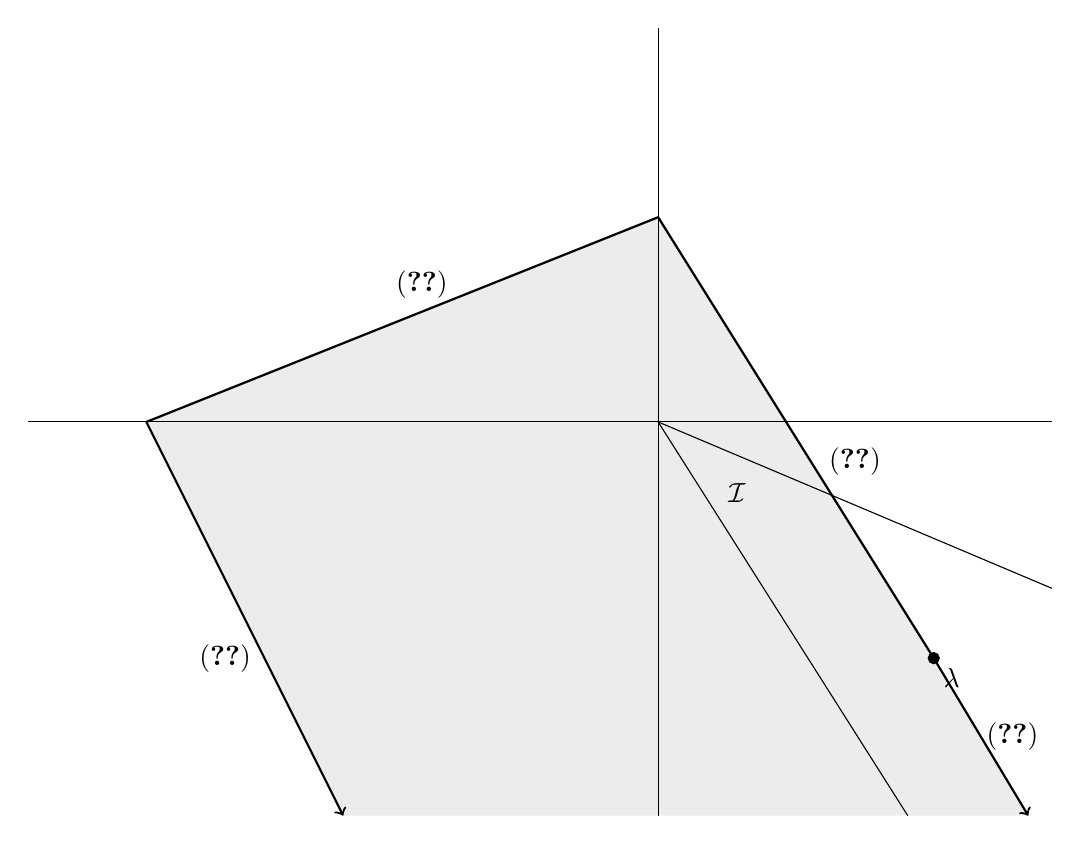
\begin{tikzpicture}
        \filldraw[color=lightgray!30] (47/10,-5) --(3.5,-3) -- (0,26/10) -- (-26/4,0) -- (-16/4,-5);
        \draw[-] (-8,0) -- (5,0);
        \draw[-] (0,-5) -- (0,5);
        %\filldraw[color=lightgray!30] (0,0) -- (5,-2.113) -- (5,-5) -- (3.17,-5) -- (0,0);
        \draw[-] (0,0) -- (5,-2.113);
        \draw[-] (0,0) -- (3.17,-5);
        \node at (1,-0.9) {$\cI$};
        \draw[fill=black] (3.5,-3) circle (2pt);
        \node[below right] at (3.5,-3) {$\lambda$};
        \draw[->,thick] (3.5,-3) -- (47/10,-5);
        \draw[-,thick] (3.5,-3) -- (0,26/10);
        \draw[-,thick] (0,26/10) -- (-26/4,0);
        \draw[->,thick] (-26/4,0) -- (-16/4,-5);
        \node at (4.5,-4) {\eqref{ineq:1}};
        \node at (2.5,-0.5) {\eqref{ineq:2}};
        \node at (-3,1.75) {\eqref{ineq:3}};
        \node at (-5.5,-3) {\eqref{ineq:4}};
      \end{tikzpicture}
    \]
  \end{lemma}
  \begin{proof}
    Following Lemma~\ref{le:imaginary transformations}, we consider even and odd sequences of mutations separately.

    For $i=2j$, $j>0$, and $\lambda\in\cI$, we observe that $\cC_{t_i}(\phi_{t_i}\lambda)\subset\RR^2$ is given by the inequalities 
    \[ (\dagger)\ x\le u_{2j+1,+}\lambda_1+u_{2j,+}\lambda_2 \qquad\text{and}\qquad (\ddagger)\ -y\le u_{2j,-}\lambda_1+u_{2j-1,-}\lambda_2. \]
    We inductively compute the region $\phi_{t_{2j}}^{-1}\cC_{t_{2j}}(\phi_{t_{2j}}\lambda)$, using Lemma~\ref{le:transformed inequalities} and the equality $\phi_{t_{2j}}^{-1}=\phi_{t_2}^{-j}$.

    \subsubsection*{Claim:} For $k>0$, $\phi_{t_{2k}}^{-1}\cC_{t_{2j}}(\phi_{t_{2j}}\lambda)$ is the region determined by the inequalities 
    \begin{align*}
      \tag{a} u_{2k,-}x+u_{2k-1,+}y &\le u_{2j,-}\lambda_1+u_{2j-1,+}\lambda_2;\\
      \tag{b} u_{2k+1,-}x+u_{2k,+}y &\le u_{2j+1,-}\lambda_1+u_{2j,+}\lambda_2;\\
      \tag{c} -u_{2k-1,-}x+u_{2k,+}y &\le u_{2j+1,-}\lambda_1+u_{2j,+}\lambda_2;\\
      \tag{d} -u_{2k-1,-}x-u_{2k-2,+}y &\le u_{2j+1,-}\lambda_1+u_{2j,+}\lambda_2.
    \end{align*}

    We see from \eqref{eq:backward two step mutation}, that $\lambda\in\cI$ implies the boundary ray for $\cC_{t_{2j}}(\phi_{t_{2j}}\lambda)$ corresponding to ($\ddagger$) lies entirely in the region in which $\phi_{t_2}^{-1}$ acts according to the matrix $\left[ \begin{array}{cc} -1 & -b\\ c & bc-1 \end{array}\right]$ of determinant 1.
    By Lemma~\ref{le:transformed inequalities}, the inequality ($\ddagger$) transforms into the inequality $cx+y\le u_{i,-}\lambda_1+u_{i-1,+}\lambda_2$ which corresponds to (a) with $k=1$.
    Similarly, the boundary ray for $\cC_{t_{2j}}(\phi_{t_{2j}}\lambda)$ corresponding to ($\dagger$) intersects three domains of linearity in which $\phi_{t_2}^{-1}$ acts according to the matrices $\left[ \begin{array}{cc} -1 & -b\\ c & bc-1 \end{array}\right]$, $\left[ \begin{array}{cc} -1 & -b\\ 0 & -1 \end{array}\right]$, $\left[ \begin{array}{cc} -1 & 0\\ 0 & -1 \end{array}\right]$, each of determinant 1.
    By Lemma~\ref{le:transformed inequalities}, the inequality ($\dagger$) can be seen to transform by these into each of inequalities (b), (c), (d) with $k=1$.
    This establishes the base of an induction on $k$.

    Assuming the inequalities (a)-(d) hold for $k$, we apply Lemma~\ref{le:transformed inequalities} with $\phi_{t_2}^{-1}$.
    Both of the boundary rays corresponding to the inequalities (a) and (d) lies entirely in the region where $\phi_{t_2}^{-1}$ acts according to the matrix $\left[ \begin{array}{cc} -1 & -b\\ c & bc-1 \end{array}\right]$, also the boundary segment corresponding to (b) intersects this region.
    Thus applying Lemma~\ref{le:transformed inequalities} to (a) gives the inequality 
    \[u_{2k+2,-}x+u_{2k+1,+}y=(u_{3,+}u_{2k,-}-u_{2,-}u_{2k-1,+})x+(u_{2,+}u_{2k,-}-u_{1,-}u_{2k-1,+})y\le u_{2j,-}\lambda_1+u_{2j-1,+}\lambda_2,\]
    which is the inequality (a) for $k+1$ by Lemma~\ref{eq:long Chebyshev recursion}; while applying this to (d) gives the inequality 
    \[-u_{2k+1,-}x-u_{2k,+}y=(-u_{3,+}u_{2k-1,-}+u_{2,-}u_{2k-2,+})x+(-u_{2,+}u_{2k-1,-}+u_{1,-}u_{2k-2,+})y\le u_{2j+1,-}\lambda_1+u_{2j,+}\lambda_2,\]
    which is the inequality (d) for $k+1$ again by Lemma~\ref{eq:long Chebyshev recursion}; finally applying this to (b) gives the inequality 
    \[u_{2k+3,-}x+u_{2k+2,+}y=(u_{3,+}u_{2k+1,-}-u_{2,-}u_{2k,+})x+(u_{2,+}u_{2k+1,-}-u_{1,-}u_{2k,+})y\le u_{2j+1,-}\lambda_1+u_{2j,+}\lambda_2,\]
    which is the inequality (b) for $k+1$.
    Similarly, the boundary segment corresponding to (c) lies entirely in the region where $\phi_{t_2}^{-1}$ acts according to the matrix $\left[ \begin{array}{cc} -1 & 0\\ c & -1 \end{array}\right]$.
    Thus applying Lemma~\ref{le:transformed inequalities} to (c) gives the inequality 
    \[-u_{2k+1,-}x-u_{2k,+}y=(u_{1,+}u_{2k-1,-}-u_{2,-}u_{2k,+})x+(-u_{0,+}u_{2k-1,-}-u_{1,-}u_{2k,+})y\le u_{2j+1,-}\lambda_1+u_{2j,+}\lambda_2,\]
    which is the inequality (d) for $k+1$ by Lemma~\ref{eq:long Chebyshev recursion}, in particular we see that the segment determined by (c) and the ray determined by (d) align in the image.
    Lastly, the boundary segment corresponding to (b) also intersects the regions where $\phi_{t_2}^{-1}$ acts according to the matrices $\left[ \begin{array}{cc} -1 & -b\\ 0 & -1 \end{array}\right]$ and $\left[ \begin{array}{cc} -1 & 0\\ 0 & -1 \end{array}\right]$ respectively.
    Applying Lemma~\ref{le:transformed inequalities} to (b) with the first matrix gives the inequality 
    \[-u_{2k+1,-}x+u_{2k+2,+}y=(-u_{1,+}u_{2k+1,-}+u_{0,-}u_{2k,+})x+(u_{2,+}u_{2k+1,-}-u_{1,-}u_{2k,+})y\le u_{2j+1,-}\lambda_1+u_{2j,+}\lambda_2,\]
    which is the inequality (c) for $k+1$ by Lemma~\ref{eq:long Chebyshev recursion}, while applying Lemma~\ref{le:transformed inequalities} to (b) with the second matrix gives the inequality 
    \[-u_{2k+1,-}x-u_{2k,+}y\le u_{2j+1,-}\lambda_1+u_{2j,+}\lambda_2,\]
    which again reproduces the inequality (d) and aligns with the previous segment and ray in the image.
    This completes the induction on $k$, proving the Claim and the result for $i$ even.

    For $i=2j+1$, $j>0$, and $\lambda\in\cI$, we get $\cC_{t_{2j+1}}(\phi_{t_{2j+1}}\lambda)\subset\RR^2$ is given by the inequalities 
    \[ (\dagger')\ -x\le u_{2j+1,+}\lambda_1+u_{2j,+}\lambda_2 \qquad\text{and}\qquad (\ddagger')\ y\le u_{2j+2,-}\lambda_1+u_{2j+1,-}\lambda_2.\]
    Using that $\phi_{t_{2j+1}}^{-1}=\phi_{t_2}^{-j}\phi_{t_1}^{-1}$, we compute the image inductively as above.
    From \eqref{eq:forward mutation 1} and Lemma~\ref{le:imaginary stability}, we see that the boundary ray for $\cC_{t_{2j+1}}(\phi_{t_{2j+1}}\lambda)$ corresponding to ($\dagger'$) lies entirely in the region in which $\phi_{t_1}^{-1}$ acts according to the matrix $\left[ \begin{array}{cc} -1 & 0\\ c & 1 \end{array}\right]$ of determinant $-1$.
    Thus applying Lemma~\ref{le:transformed inequalities}, the inequality ($\dagger'$) is transformed by $\phi_{t_1}^{-1}$ into the inequality $x\le u_{2j+1,+}\lambda_1+u_{2j,+}\lambda_2$.
    The boundary ray corresponding to ($\ddagger'$) intersects both domains of linearity for $\phi_{t_1}^{-1}$ and thus produces the inequalities
    \[ cx+y\le u_{2j+2,+}\lambda_1+u_{2j+1,+}\lambda_2 \qquad\text{and}\qquad  y\le u_{2j+2,+}\lambda_1+u_{2j+1,+}\lambda_2.\]


    \subsubsection*{Claim:} For $k\ge 0$, $\phi_{t_{2k+1}}^{-1}\cC_{t_{2j+1}}(\phi_{t_{2j+1}}\lambda)$ is the region determined by the inequalities 
    \begin{align*}
      \tag{a$'$} u_{2k+1,-}x+u_{2k,+}y &\le u_{2j+1,-}\lambda_1+u_{2j,+}\lambda_2;\\
      \tag{b$'$} u_{2k+2,-}x+u_{2k+1,+}y &\le u_{2j+2,-}\lambda_1+u_{2j+1,+}\lambda_2;\\
      \tag{c$'$} -u_{2k,-}x+u_{2k+1,+}y &\le u_{2j+2,-}\lambda_1+u_{2j+1,+}\lambda_2;\\
      \tag{d$'$} -u_{2k,-}x-u_{2k-1,+}y &\le u_{2j+2,-}\lambda_1+u_{2j+1,+}\lambda_2.
    \end{align*}
    By essentially the same calculations as above, these inequalities reproduce under the action of $\phi_{t_2}^{-1}$ and this completes the proof.
  \end{proof}

  The standard Chebyshev polynomials (of the second kind) are defined by the recursion $u_{i+1}=ru_i-u_{i-1}$, $u_1=1$, $u_0=0$, which can be computed explicitly as
  \[u_i(r)=\frac{1}{2^i\sqrt{r^2-4}}\left(\big(r+\sqrt{r^2-4}\big)^i-\big(r-\sqrt{r^2-4}\big)^i\right).\]
  By the equalities 
  \[u_{i,\varepsilon}=\begin{cases} \frac{\sqrt{b}}{\sqrt{c}}u_i(\sqrt{bc}) & \text{if $i$ is even and $\varepsilon=+$;}\\ \frac{\sqrt{c}}{\sqrt{b}}u_i(\sqrt{bc}) & \text{if $i$ is even and $\varepsilon=-$;}\\ u_i(\sqrt{bc}) & \text{if $i$ is odd;} \end{cases}\]
  it follows that $u_{i,\varepsilon}$ can be computed explicitly as
  \[u_{i,\varepsilon}=\begin{cases} \frac{\sqrt{b}}{2^i\sqrt{c(bc-4)}}\left(\big(\sqrt{bc}+\sqrt{bc-4}\big)^i-\big(\sqrt{bc}-\sqrt{bc-4}\big)^i\right) & \text{if $i$ is even and $\varepsilon=+$;}\\ \frac{\sqrt{c}}{2^i\sqrt{b(bc-4)}}\left(\big(\sqrt{bc}+\sqrt{bc-4}\big)^i-\big(\sqrt{bc}-\sqrt{bc-4}\big)^i\right) & \text{if $i$ is even and $\varepsilon=-$;}\\ \frac{1}{2^i\sqrt{bc-4}}\left(\big(\sqrt{bc}+\sqrt{bc-4}\big)^i-\big(\sqrt{bc}-\sqrt{bc-4}\big)^i\right) & \text{if $i$ is odd.} \end{cases}\]
  \begin{remark}
    Note that $u_{2j+1,+}=u_{2j+1,-}$ for all $j\in\ZZ$.
    Moreover, since $u_{-i,\varepsilon}=-u_{i,\varepsilon}$, these formulas can also easily be seen to hold for $i<0$.
  \end{remark}

  \begin{lemma}
    We have
    \[\lim_{i\to\infty} \frac{-u_{i,-}}{u_{i-1,+}}=\frac{-bc-\sqrt{bc(bc-4)}}{2b} \qquad \lim_{i\to\infty} \frac{-u_{i-1,-}}{u_{i,+}}=\frac{-bc+\sqrt{bc(bc-4)}}{2b}.\]
  \end{lemma}
  \begin{proof}
    For any $i\ge 1$, we have
    \[\frac{\big(\sqrt{bc}+\sqrt{bc-4}\big)^i-\big(\sqrt{bc}-\sqrt{bc-4}\big)^i}{\big(\sqrt{bc}+\sqrt{bc-4}\big)^{i-1}-\big(\sqrt{bc}-\sqrt{bc-4}\big)^{i-1}}=\frac{\sqrt{bc}+\sqrt{bc-4}}{1-\left(\frac{\sqrt{bc}-\sqrt{bc-4}}{\sqrt{bc}+\sqrt{bc-4}}\right)^{i-1}}.\]
    It follows that
    \[\lim_{i\to\infty} \frac{-u_{i,-}}{u_{i-1,+}} = \lim_{i\to\infty} \left( \frac{-\sqrt{c}}{2\sqrt{b}}\cdot\frac{\sqrt{bc}+\sqrt{bc-4}}{1-\left(\frac{\sqrt{bc}-\sqrt{bc-4}}{\sqrt{bc}+\sqrt{bc-4}}\right)^{i-1}} \right) = \frac{-\sqrt{c}}{2\sqrt{b}}\cdot\big(\sqrt{bc}+\sqrt{bc-4}\big),\]
    which is equivalent to the desired expression.
    Similarly, 
    \[\frac{\big(\sqrt{bc}+\sqrt{bc-4}\big)^{i-1}-\big(\sqrt{bc}-\sqrt{bc-4}\big)^{i-1}}{\big(\sqrt{bc}+\sqrt{bc-4}\big)^i-\big(\sqrt{bc}-\sqrt{bc-4}\big)^i}=\frac{\sqrt{bc}-\sqrt{bc-4}}{4\left(1-\left(\frac{\sqrt{bc}-\sqrt{bc-4}}{\sqrt{bc}+\sqrt{bc-4}}\right)^i\right)},\]
    so that
    \[\lim_{i\to\infty} \frac{-u_{i-1,-}}{u_{i,+}} = \lim_{i\to\infty} \left( \frac{-2\sqrt{c}}{\sqrt{b}}\cdot\frac{\sqrt{bc}-\sqrt{bc-4}}{4\left(1-\left(\frac{\sqrt{bc}-\sqrt{bc-4}}{\sqrt{bc}+\sqrt{bc-4}}\right)^{i-1}\right)} \right) = \frac{-\sqrt{c}}{2\sqrt{b}}\cdot\big(\sqrt{bc}-\sqrt{bc-4}\big),\]
    which is again equivalent to the desired expression.
  \end{proof}

  \begin{lemma}
    If $\lambda\in\ZZ^2\setminus\cI$, then $\cP(\lambda)=\{\lambda\}$.
  \end{lemma}
  \begin{proof}
    It is enough to consider $\phi_{t_{-2}}^{-1}\cC(\phi_{t_{-2}}\lambda) \cap \cC(\lambda) \cap \phi_{t_2}^{-1}\cC(\phi_{t_2}\lambda)$, we leave the details to the reader.
  \end{proof}

  \begin{lemma}
    \label{le:one direction}
    For $\lambda\in\cI\cap\ZZ^2$, 
    \begin{enumerate}
      \item $\cP_+(\lambda):=\bigcap_{i \ge 0}\phi_{t_i}^{-1}\cC(\phi_{t_i}\lambda)$ is the quadrilateral with corner vertices $\lambda$, $(\frac{2-bc-\sqrt{bc(bc-4)}}{2}\lambda_1-\frac{bc+\sqrt{bc(bc-4)}}{2c}\lambda_2,0)$, $(0,\frac{bc+\sqrt{bc(bc-4)}}{2b}\lambda_1+\lambda_2)$, and $(\frac{2-bc-\sqrt{bc(bc-4)}}{2}\lambda_1-b\lambda_2,\lambda_2)$.
      \item $\cP_-(\lambda):=\bigcap_{i \le 0}\phi_{t_i}^{-1}\cC(\phi_{t_i}\lambda)$ is the quadrilateral with corner vertices $\lambda$, $(\lambda_1+\frac{bc+\sqrt{bc(bc-4)}}{2c}\lambda_2,0)$, $(0,-\frac{bc+\sqrt{bc(bc-4)}}{2b}\lambda_1+\frac{2-bc-\sqrt{bc(bc-4)}}{2}\lambda_2)$, and $(\lambda_1,-c\lambda_1+\frac{2-bc-\sqrt{bc(bc-4)}}{2}\lambda_2)$.
    \end{enumerate}
  \end{lemma}
  \begin{proof}
    We prove (1) as (2) is obtained by interchanging $b$ with $c$ and swapping all ordered pairs.  
    We first show that $\cC(\lambda) \cap \phi_{t_i}^{-1}\cC(\phi_{t_i}\lambda)\supsetneq \cC(\lambda) \cap \phi_{t_j}^{-1}\cC(\phi_{t_j}\lambda)$ for $0\le i<j$.
  \end{proof}

  \begin{theorem}
    For $\lambda\in\cI\cap\ZZ^2$, there are five classes of dominance polytopes.
    \begin{enumerate}
      \item if $\lambda$ lies in the interior of the cone spanned by the vectors $(2b,-bc-\sqrt{bc(bc-4)})$ and $(2,-c)$, then $\cC(\lambda)$ is the trapezoid with corner vertices $\lambda$, $(\frac{2-bc-\sqrt{bc(bc-4)}}{2}\lambda_1-\frac{bc+\sqrt{bc(bc-4)}}{2c}\lambda_2,0)$, $(0,\frac{bc+\sqrt{bc(bc-4)}}{2b}\lambda_1+\lambda_2)$, and ???.
      \item if $\lambda$ lies on the ray spanned by $(2,-c)$, say $\lambda=(2\ell,-c\ell)$, then $\cC(\lambda)$ is the triangle with corner vertices $\lambda$, $(2\ell-\frac{bc+\sqrt{bc(bc-4)}}{2}\ell,0)$, and $(0,\frac{\sqrt{bc(bc-4)}}{b}\ell)$.
      \item if $\lambda$ lies in the interior of the cone spanned by the vectors $(2,-c)$ and $(b,-2)$, then $\cC(\lambda)$ is the kite with corner vertices $\lambda$, $(\lambda_1+\frac{bc+\sqrt{bc(bc-4)}}{2c}\lambda_2,0)$, $\frac{bc+\sqrt{bc(bc-4)}}{2\sqrt{bc(bc-4)}}(2\lambda_1+b\lambda_2,c\lambda_1+2\lambda_2)$, and $(0,\frac{bc+\sqrt{bc(bc-4)}}{2b}\lambda_1+\lambda_2)$.
      \item if $\lambda$ lies on the ray spanned by $(b,-2)$, say $\lambda=(b\ell,-2\ell)$, then $\cC(\lambda)$ is the triangle with corner vertices $\lambda$, $(-\frac{\sqrt{bc(bc-4)}}{c}\ell,0)$, and $(0,\frac{bc+\sqrt{bc(bc-4)}}{2}\ell-2\ell)$.
      \item if $\lambda$ lies in the interior of the cone spanned by the vectors $(b,-2)$ and $(2b,-bc+\sqrt{bc(bc-4)})$, then $\cC(\lambda)$ is the triangle with corner vertices $\lambda$, $(\lambda_1+\frac{bc+\sqrt{bc(bc-4)}}{2c}\lambda_2,0)$, $(0,-\frac{bc+\sqrt{bc(bc-4)}}{2b}\lambda_1+\frac{2-bc-\sqrt{bc(bc-4)}}{2}\lambda_2)$, and ???.
    \end{enumerate}
  \end{theorem}
  \begin{proof}
    Following Lemma~\ref{le:one direction}, we see that the intersection $\cP_+(\lambda)\cap\cP_-(\lambda)$ degenerates to a triangle precisely when
    \[\frac{2-bc-\sqrt{bc(bc-4)}}{2}\lambda_1-\frac{bc+\sqrt{bc(bc-4)}}{2c}\lambda_2=\lambda_1+\frac{bc+\sqrt{bc(bc-4)}}{2c}\lambda_2\]
    or 
    \[\frac{bc+\sqrt{bc(bc-4)}}{2b}\lambda_1+\lambda_2=-\frac{bc+\sqrt{bc(bc-4)}}{2b}\lambda_1+\frac{2-bc-\sqrt{bc(bc-4)}}{2}\lambda_2.\]
    The first equations reduces to $c\lambda_1+2\lambda_2=0$, while the second reduces to $2\lambda_1+b\lambda_2=0$.
    In particular, the rays spanned by $(2,-c)$ and $(b,-2)$ determine this change of state in the dominance regions $\cP(\lambda)$.
  \end{proof}

  \begin{remark}
    Note that the rays which separate the regions inside $\cI$ correspond exactly to the columns of the associated Cartan matrix $\left[ \begin{array}{cc} 2 & -b \\ -c & 2 \end{array} \right]$.
    This unexpected coincidence is one of our reasons for deciding to write down these results.
  \end{remark}

  The dominance polygon pointed at $\lambda=(\lambda_1,\lambda_2)$ is the region defined by the following six inequalities:
  \begin{align}
    -\lambda_1-\frac{b c+\sqrt{b c (b c-4)}}{2 c}\lambda_2+x+\frac{b c+\sqrt{b c (b c-4)}}{2 c}y\geq0
    \\
    \frac{b c+\sqrt{b c (b c-4)}}{2 b}\lambda_1+\lambda_2-\frac{b c+\sqrt{b c (b c-4)}}{2 b}x-y\geq0
    \\
    -\frac{b c+\sqrt{b c (b c-4)}}{2 b}\lambda_1 - \frac{b c+\sqrt{b c (b c-4)}-2}{2}\lambda_2 + \frac{b c+\sqrt{b c (b c-4)}}{2 b}x-y\geq0
    \\
    \frac{b c+\sqrt{b c (b c-4)}-2}{2}\lambda_1+\frac{b c+\sqrt{b c (b c-4)}}{2 c}\lambda_2+x-\frac{b c+\sqrt{b c (b c-4)}}{2 c}y\geq0
    \\
    -\frac{b c+\sqrt{b c (b c-4)}}{2 b}\lambda_1-\frac{b c+\sqrt{b c (b c-4)}-2}{2}\lambda_2-\frac{b c-\sqrt{b c (b c-4)}}{2 b}x-y\geq0
    \\
    \frac{b c+\sqrt{b c (b c-4)}-2}{2}\lambda_1+\frac{b c+\sqrt{b c (b c-4)}}{2 c}\lambda_2+x+\frac{b c-\sqrt{b c (b c-4)}}{2 c}y\geq0
  \end{align}
  Are any of these better forms?
  \begin{align}
    (x-\lambda_1)+\frac{b c+\sqrt{b c (b c-4)}}{2 c}(y-\lambda_2)\geq0
    \\
    \nonumber \iff \frac{b c-\sqrt{b c (b c-4)}}{2 b}(x-\lambda_1)+(y-\lambda_2)\geq0
    \\
    -\frac{b c+\sqrt{b c (b c-4)}}{2 b}(x-\lambda_1)-(y-\lambda_2)\geq0
    \\
    \nonumber \iff -(x-\lambda_1)-\frac{b c-\sqrt{b c (b c-4)}}{2 c}(y-\lambda_2)\geq0
    \\
    -\frac{b c+\sqrt{b c (b c-4)}}{2}\lambda_2 + \frac{b c+\sqrt{b c (b c-4)}}{2 b}(x-\lambda_1)-(y-\lambda_2)\geq0
    \\
    \nonumber \iff -b\lambda_2 + (x-\lambda_1)-\frac{b c-\sqrt{b c (b c-4)}}{2 c}(y-\lambda_2)\geq0
    \\
    \frac{b c+\sqrt{b c (b c-4)}}{2}\lambda_1+(x-\lambda_1)-\frac{b c+\sqrt{b c (b c-4)}}{2 c}(y-\lambda_2)\geq0
    \\
    \nonumber \iff c\lambda_1+\frac{b c-\sqrt{b c (b c-4)}}{2 b}(x-\lambda_1)-(y-\lambda_2)\geq0
    \\
    -c\lambda_1-\frac{b c+\sqrt{b c (b c-4)}}{2}\lambda_2-\frac{b c-\sqrt{b c (b c-4)}}{2 b}(x-\lambda_1)-(y-\lambda_2)\geq0
    \\
    \frac{b c+\sqrt{b c (b c-4)}}{2}\lambda_1+b\lambda_2+(x-\lambda_1)+\frac{b c-\sqrt{b c (b c-4)}}{2 c}(y-\lambda_2)\geq0
  \end{align}
  Another proposal (I also changed the order of the equations)
  \begin{align}
    \frac{b c-\sqrt{b c (b c-4)}}{2 b}(x-\lambda_1)+(y-\lambda_2) & \geq0
    \\
    \frac{b c+\sqrt{b c (b c-4)}}{2 b}(x-\lambda_1)-(y-\lambda_2) & \geq \frac{b c+\sqrt{b c (b c-4)}}{2b}b\lambda_2 
    \\
    -\frac{b c-\sqrt{b c (b c-4)}}{2 b}(x-\lambda_1)-(y-\lambda_2)& \geq c\lambda_1+\frac{b c+\sqrt{b c (b c-4)}}{2b}b\lambda_2
    \\
    -(x-\lambda_1)-\frac{b c-\sqrt{b c (b c-4)}}{2 c}(y-\lambda_2)& \geq0
    \\
    (x-\lambda_1)-\frac{b c+\sqrt{b c (b c-4)}}{2 c}(y-\lambda_2) & \geq -\frac{b c+\sqrt{b c (b c-4)}}{2c}c\lambda_1
    \\
    (x-\lambda_1)+\frac{b c-\sqrt{b c (b c-4)}}{2 c}(y-\lambda_2) & \geq -\frac{b c+\sqrt{b c (b c-4)}}{2c}c\lambda_1-b\lambda_2
  \end{align}



  \subsection{Deformation Support}
  The greedy basis of Lee, Li, and Zelevinsky \cite{???} can be defined as the positive pointed basis with minimal support.
  Here we identify the maximum possible support of its deformations.

  Consider the deformation of the theta basis element with $\bfg$-vector $\lambda$.
  \begin{theorem}
    For $\lambda\in\cI\cap\ZZ^2$, the support of any deformation of the corresponding theta basis element is contained in the polytope defined by the following inequalities:
    \begin{align*}
       \lambda_1-b\lambda_2 &\le x\\
       \lambda_2 &\le y\\
    \end{align*}
    is the convex hull of the following vertices:
    \[\lambda, \qquad (\lambda_1-b\lambda_2,\lambda_2), \qquad (\lambda_1-b\lambda_2,\lambda_2-c\lambda_1), \qquad (?,?)\]
    The $d$-vector is $(\lambda_1-b\lambda_2,\lambda_2)$

    $\frac{bc+\sqrt{bc(bc-4)}}{2\sqrt{bc(bc-4)}}(2\lambda_1+b\lambda_2,c\lambda_1+2\lambda_2)$, and $(0,\frac{bc+\sqrt{bc(bc-4)}}{2b}\lambda_1+\lambda_2)$

    Slope:
    \[\big(\frac{bc+\sqrt{bc(bc-4)}}{2\sqrt{bc(bc-4)}}(c\lambda_1+2\lambda_2)-(\frac{bc+\sqrt{bc(bc-4)}}{2b}\lambda_1+\lambda_2)\big) /\frac{bc+\sqrt{bc(bc-4)}}{2\sqrt{bc(bc-4)}}(2\lambda_1+b\lambda_2)\]

    $y=$

    $(\lambda_1,\lambda_2)$ and $(0,\frac{bc+\sqrt{bc(bc-4)}}{2b}\lambda_1+\lambda_2)$
    
    Slope: $-\frac{bc+\sqrt{bc(bc-4)}}{2b}$\\

    Corner of dominant support?: 
    \begin{align*}
      \left(\frac{bc+\sqrt{bc(bc-4)}}{2\sqrt{bc(bc-4)}}(2\lambda_1+b\lambda_2),-\frac{bc+\sqrt{bc(bc-4)}}{2b}\frac{bc+\sqrt{bc(bc-4)}}{2\sqrt{bc(bc-4)}}(2\lambda_1+b\lambda_2)+\frac{bc+\sqrt{bc(bc-4)}}{2b}\lambda_1+\lambda_2\right)\\
      \left(\frac{bc+\sqrt{bc(bc-4)}}{2\sqrt{bc(bc-4)}}(2\lambda_1+b\lambda_2),-\frac{bc+\sqrt{bc(bc-4)}}{2b}\frac{bc}{\sqrt{bc(bc-4)}}\lambda_1+-\frac{bc+\sqrt{bc(bc-4)}}{2}\frac{bc+\sqrt{bc(bc-4)}}{2\sqrt{bc(bc-4)}}\lambda_2+\lambda_2\right)\\
    \end{align*}
    
  \end{theorem}


  \section{The Total Domination Polyhedron}

  Define the \emph{total domination polyhedron} $\cD:=\{(\lambda,\mu):\mu\in\cP(\lambda)\}$, i.e. this is the set of all pairs where $\lambda$ dominates $\mu$.
  Write $\pi_1:\cD\to\RR^n$ for the projection to $\lambda$ and $\pi_2:\cD\to\RR^n$ for the projection to $\mu$.
  \begin{itemize}
    \item Is it a polyhedron?
    \item The lemma below might suggest so.  
      Indeed, if it is, by the Decomposition Theorem, we can write $\cD$ as the Minkowski sum of a polyhedral cone (almost certainly $\cI$) and a convex polytope (what is it?).
      I am ignoring that it should really be the union of this polyhedron with a plane if the previous sentence holds any water.
    \item Actually, we might need to take the union of several polyhedra to account for the variations in the fibers $\pi_1^{-1}(\lambda)$.
  \end{itemize}

  Is the following result true beyond rank 2?
  \begin{lemma}
    For $\mu\in\RR^2$, $\pi_2^{-1}(\mu)$ is a translate of the imaginary cone $\cI$ or the union of such with a single point.
  \end{lemma}
  \begin{proof}
    For $\mu$ in the second quadrant, the vertex of this cone should be given by $\lambda=(\lambda_1,\lambda_2)$ where
    \[\lambda_1=\frac{2b\mu_2-4\mu_1}{bc-4+\sqrt{bc(bc-4)}} \qquad \text{and} \qquad \lambda_2=\frac{2c\mu_1-4\mu_2}{bc-4+\sqrt{bc(bc-4)}}.\]
    (This comes from setting $\mu$ to be the vertex opposite $\lambda$ inside the dominance region $\cP(\lambda)$ and then solving for $\lambda$.)
  \end{proof}
  \begin{remark}
    We want to understand what the curve is that results when we have $\mu$ lie along the unit circle, this should be possible by plugging $(\cos(\theta),\sin(\theta))$ into this formula for $\lambda$ and seeing what ellipse we get.
  \end{remark}


  \section{Ignore}
  Rank 4 Skew-Symmetric $B$

  $P(\lambda)=\lambda^4 + a\lambda^3 + b\lambda^2 + c\lambda + 1$

  \begin{align*}
    a
    &=-b_{41}b_{21}b_{32}b_{43}-b_{31}b_{21}b_{32}-b_{41}b_{21}b_{42}-b_{41}b_{31}b_{43}-b_{42}b_{32}b_{43}-b_{21}b_{21}-b_{31}b_{31}-b_{32}b_{32}-b_{41}b_{41}-b_{42}b_{42}-b_{43}b_{43}+4\\
    c
    &=-b_{21}b_{32}b_{43}b_{41}-b_{21}b_{32}b_{31}-b_{21}b_{42}b_{41}-b_{31}b_{43}b_{41}-b_{32}b_{43}b_{42}-b_{21}b_{21}-b_{31}b_{31}-b_{32}b_{32}-b_{41}b_{41}-b_{42}b_{42}-b_{43}b_{43}+4\\
    b
    &=b_{41} b_{32} b_{32} b_{41} - b_{31} b_{42} b_{32} b_{41} - b_{31} b_{43} b_{21} b_{42} - b_{41} b_{32} b_{31} b_{42} + b_{31} b_{42} b_{31} b_{42} + b_{21} b_{43} b_{21} b_{43} - b_{21} b_{42} b_{31} b_{43}\\
    &\quad - b_{21} b_{32} b_{31} - b_{31} b_{21} b_{32} - b_{21} b_{42} b_{41} - b_{31} b_{43} b_{41} - b_{32} b_{43} b_{42} - b_{41} b_{21} b_{42} - b_{41} b_{31} b_{43} - b_{42} b_{32} b_{43}\\
    &\quad - 2 b_{21} b_{21} - 2 b_{31} b_{31} - 2 b_{32} b_{32} - 2 b_{41} b_{41} - 2 b_{42} b_{42} - 2 b_{43} b_{43} + 6\\
    &=a+c-2+m\\
    &=a+c-2+n^2\\
    m
    &=b_{41}b_{21}b_{32}b_{43}+b_{21}b_{32}b_{43}b_{41}+b_{41}b_{32}b_{32}b_{41}-b_{31}b_{42}b_{32}b_{41}-b_{31}b_{43}b_{21}b_{42}-b_{41}b_{32}b_{31}b_{42}+b_{31}b_{42}b_{31}b_{42}+b_{21}b_{43}b_{21}b_{43}\\
    &\quad -b_{21}b_{42}b_{31}b_{43}\\
    &=(b_{31}b_{42}-b_{32}b_{41}-b_{21}b_{43})^2\\
    n
    &=b_{31}b_{42}-b_{32}b_{41}-b_{21}b_{43}\\
  \end{align*}

  Observe that $P(-1)=n^2$.
  What happens when $\lambda=\frac{-a\pm\sqrt{a^2-4}}{2}$?  You get $P(\lambda)=(b-2)\lambda^2$.
    
\end{document}
